% !TeX encoding = UTF-8
% !TeX root = ../main.tex
% !TeX spellcheck = en_US
\chapter{Work}
\label{cha:work}

This chapter describes the experiments and approaches tried and implemented during the thesis. It should give a description about the decisions made and the problems occurred based on the decisions and implementation limitations.

\section{Extracting features}

The image feature were represented by \acf{HOG} (as described in \prettyref{sec:hog})

\section{Abstracting the feature computation}

One of the initial steps made was to find a way to represent a collection of extracted features (as taken from a part candidate or a query image). This should enable the precomputation of the image database and also create a similarity linkage right away into the stored database.

To fulfill these requirements, the decision goes to try to cluster the features with a k-means clustering (see \prettyref{sec:kmeans}) or a fisher vector representation (see \prettyref{sec:fisher}) based on a \acf{GMM} (see \prettyref{sec:gmm}).
\par
The initial experiments were used to detect if codebooks based on clustered features could be used to express similarities among different candidates. This was done by using the bicycle and car classes of the \ac{VOC2011} Image database \cite{Pascal2011}.
The clustering was initially done with 512, 1000 and 3000 k-means and 128, 256 and 384 \ac{GMM} clusters over all features extracted from the \ac{VOC2011} bicycle and car trainval image classes.
At this point all experiments were done by using normal \ac{HOG} and whiten \ac{HOG} (see \prettyref{sec:whitened_hog}) for performance comparison.
\par
The low-level \ac{HOG} implementation is provided by the Exemplar-SVM framework \cite{Malisiewicz2011}. This implementation produces a feature pyramid with $31$ dimensional features at different scales $S$.

\begin{equation}
S = \{s|s = \frac{1}{2^{0.1 * (i-1)}}; i \in \mathbb{N}; 1 \le i \le 100;\}
\end{equation}

For each level of the pyramid, the input image will be rescaled by the corresponding scale factor $s$, until no features could be extracted or the rescaled image contains less than 5 pixel per dimension.
\par
The calculated pyramid is then transfered in a list of feature vectors and their corresponding bounding boxes. This is done by combining the given features at each level of the pyramid into $5\times5$ grids and reshaping them into $775$ dimensional vectors.
As the experiments were executed with labeled bounding boxes, unnecessary features had to be removed from the list. This is achieved by specifying a pixel-wise boolean mask $M_p$ for the desired image regions. The mask will be transformed into a cell-wise $M_c$ at each scale $s$. This is done by a standard bicubic kernel convolution as in \eqnref{bicubic_kernel}.

\begin{equation}
k_x = \begin{cases}
(a+2)|x|^3-(a+3)|x|^2+1 & \text{for } |x| \leq 1 \\
a|x|^3-5a|x|^2+8a|x|-4a & \text{for } 1 < |x| < 2 \\
0                       & \text{otherwise}
\end{cases}
\label{eqn:bicubic_kernel}
\end{equation}

with $a=-0.5$ in the \MATLAB implementation\footnote{Implemented in the \textit{toolbox/images/images/imresize.m} file in the \MATLAB installation directory}. With this mask, all feature patches which are not fully covered by the mask were discarded.
\par
For the initial tests, a simple \acf{NN} approach with euclidean distances were used to compute the similarity between different codebooks.

This was done by selecting each labeled bounding box of each test image, computing the features $X$ (\ac{HOG} and whitened \ac{HOG}), assign them to the clusters by the corresponding centroids $C$ (either \ac{NN} in terms of k-means or by computing the fisher vector) and comparing it to the codebooks of the remaining image bounding boxes. The codebook values itself depend on the distances of the features to their corresponding centroids as described in \prettyref{eqn:codebook_calc}.

%TODO algorithm or formular???
%\begin{algorithm}
%	\KwIn{$X$: Features extracted from a bounding box, $C$: Cluster centroids}
%	\KwOut{$c$: codebook representing the given features}
%	\KwData{$D$: distance vector of each feature to its nearest centroid, $I$: assignment vector of each feature to its nearest centroid}
%	$D, I \gets \text{NearestNeighbourSearch}(X, C)$\;
%	
%	\ForEach{$d$ of $D$ and $i$ of $I$}{
%		$c_i \gets c_i + \frac{1}{d}$\;
%	}
%	\caption{Computing codebook from features}
%	\label{alg:codebook_calc}
%\end{algorithm}

\begin{align}
	I_j &= \arg \min_i ||X_j - C_i||_2 \\
	D_j &= \min_i ||X_j - C_i||_2 \\
	c_i &= \sum_{I_j = i} \frac{1}{D_j}
	\label{eqn:codebook_calc}
\end{align}

For a visual verification, the 15 nearest parts were shown aside to the query image. The distance between two different codebooks $c_1$ and $c_2$ was computed by the euclidean distance equation $||c_1-c_2||_2$.
%TODO beispiel bild
% searching for representative clusters (nn-iter)
For each query image, the most shared codebook dimensions and their respective patches were marked inside the images. It could be clearly seen that the patches with a comparable visual representation share the same cluster and (from a human perspective) seem to be representative for the chosen object class.
%TODO Bild mit markierung, oder auf vorheriges verweisen
To prove this assumption, an iterative \ac{NN} was implemented. It consists of several rounds, each executing a \ac{NN} search over the available patches and sorting the results. After each round, the most common codebook dimensions of the first $k$ patches were taken whilst the remaining ones were removed (set to zero) as described by \prettyref{alg:iterative_nn}.

\begin{algorithm}
	\SetKwProg{Fn}{Function}{}{end}
	\Fn{IterNearestNeighbour($q$ : query codebook, $R$ : remaining codebooks, k)}{
		\Repeat{no changes}{
			$D \gets \text{NearestNeighbourSearch}(R, q)$\;
			
			Sort $R$ based on $D$\;
			
			\tcc{$ij$ denotes dimension $i$ in codebook $j$}
			
			$S = \{i | \forall R_{ij} \ne 0; 0 < j < k\}$\;
			
			$R \gets R_{ij}$ set to $0$ if $i \notin S$\;
		}
		\Return{Sorted $R$}
	}
	\caption{Iterative \ac{NN}}
	\label{alg:iterative_nn}
\end{algorithm}

By using this algorithm, it could be shown that the most representative patches were assigned to the same clusters, as more similar objects are pulled together at each iteration.
%TODO bilder fuer verschiedene iterationen 

\par
% maintaining location information (parts)
As the reduction of several feature vectors to a single codebook for a whole bounding box eliminates the locational information, the implementation was extended to maintain some locational information by splitting the bounding box in several parts and computing a codebook for each of them. Afterwards, these codebooks are concatenated, which means that the size of a representative codebook for a whole bounding box is calculated by $numberOfParts * numberOfDimensions$. This change brought additional performance gains in terms of detecting similar parts, but also increased the memory usage significantly. During the rest of the experiments, the bounding boxes were either split into a two-by-two grid (as it seemed to be the best mix of performance gain and memory usage) or left complete for later comparisons.

\section{Scoring the part candidates}

% svm

As the direct comparison via a \ac{NN} approach did not provided the desired performance and also resulted in a time consuming task if the amount of codebooks increases, another approach was required. One possible solution for detecting similar vectors is a \ac{SVM} based classifier (for a more detailed description about \acp{SVM} see \prettyref{sec:svm}). In this particular case a C-SVC classifier was trained \cite{boser1992training} \cite{cortes1995support}.
%In this particular case a one-vs-call classifier was used. In this type only one classifier is trained to determine if a given vector is part of one class or part of all other possible classes.
The positive class is represented by the query codebook, whilst all other classes are represented by a previously collected list of codebooks. To generate this list, a set of sliding windows were calculated for each image in the database based on algorithm \ref{alg:calc_windows}.

\begin{algorithm}
    \KwIn{$I$: image}
    \KwOut{calculated windows}
    $w_I \gets \text{width of }I$\;
    $h_I \gets \text{height of }I$\;
    $S \gets \{s^2 | s \in \mathbb{N}, s \le 10 \}$\;
    $x \gets \{1, 11, 21, 31,\dots, w_I\}$\;
    $y \gets \{1, 11, 21, 31,\dots, h_I\}$\;
    \Repeat{$w_w >= w_I$ or $h_w >= h_I$ or no elements left in $S$}{
        $currentScale \gets \text{next element of }S$\;
        $w_w \gets 32 * currentScale$\;
        $h_w \gets 32 * currentScale$\;
        
        \ForEach{Combination $x_i, y_i$ of $x$ and $y$}{
            Add window $x_i, y_i, x_i + w_w, y_i + h_w$ to the list\;
        }
    }
    \caption{Calculation of sliding windows}
    \label{alg:calc_windows}
\end{algorithm}

With this list, all feature patches are assigned to these windows where their center is placed in. For each window, a codebook is calculated by equation \ref{eqn:codebook_calc}. The resulting list of codebooks is stored and loaded during the \ac{SVM} training and used as the negative training set. The \ac{SVM} training was done by the libsvm library \cite{Chang:2011:LLS:1961189.1961199} by using the \texttt{svmtrain} function. The parameters for the training are the same as for the ExemplarSVM library \cite{Malisiewicz2011} (see table \ref{tab:libsvm_train_params}).

\begin{table}
    \begin{tabular}{|l|l|}
        \hline
        \textbf{Parameter} & \textbf{Value} \\ 
        \hline
        SVM-Type           & C-SVC \\ 
        \hline
        Kernel-Type        & Linear ($u^T*v$) \\ 
        \hline
        Cost ($C$ of C-SVC)  & $0.01$ \\ 
        \hline
        Weight of positive sample ($weight*C$) & $50$ \\ 
        \hline
    \end{tabular}
    \caption{libsvm parameters}
    \label{tab:libsvm_train_params}
\end{table}

Other assignment methods were also evaluated, including multi assignments like assigning a feature to every window were a corner is located in, or to every window which contains a minimum amount of the patch (e.g. 30\% of its area). These approaches did not provide enough performance gain in comparison to the computational overhead. Another approach was the usage of the bottom right corner, which obviously led to the fact that the detection candidates were slightly shifted to the bottom right compared to an optimum detection. 

In the first place, the classification function provided by libsvm\footnote{\texttt{svmpredict(\dots)}} was used. With an increasing amount of codebooks which have to be classified by the \ac{SVM}, the function toked a big part of the computation time. By replacing the function with the \MATLAB implementation ($codebooks * (svm_{vectors}^T * svm_{coefficents}) - svm_{\rho}$) (see \prettyref{lst:matlab_svm_predict}), the computation time could be reduced from approximate 150 seconds to 3 seconds with 250,000 codebooks (5,000 windows in 50 images).

\begin{listing}
\begin{minted}{matlab}
weights = m.SVs' * m.sv_coef;

if size(codebooks, 2) == size(weights, 1)
    scores = codebooks * weights - m.rho;
else
    scores = codebooks' * weights - m.rho;
end
nans = isnan(scores);
debg('%d NaNs produced!', sum(nans))
scores(nans) = -999;
\end{minted}
\caption{\MATLAB variant of svmpredict}
\label{lst:matlab_svm_predict}
\end{listing}

\section{Reducing the computational overhead}

% integral image
During the shift from the initial tests involving the usage of labeled bounding boxes to the actual requirement of finding parts inside of image databases, the amount of computational overhead increased significantly as it requires to compute sliding windows on each image in the database and their codebooks respectively.

Therefore the idea came up to precompute the codebooks and only load them at runtime for comparison. One solution would be to compute a set of possible windows and their codebooks. At query time the best matching window ratios could be loaded and compared to the query codebook. Unfortunately was the performance dramatically decreased with this approach.

The second solution was to create integral images based on codebooks. Integral images were described by Viola and Jones in 2001 \cite{viola2001rapid}. Such images are created by summing up all pixel values from the top left to the bottom right (or any other diagonal direction). The advantage of this approach is the possibility to compute a sum value for a rectangular area by summing and subtracting the values of the four corners as described in figure \ref{fig:integral_image}. 

\begin{figure}
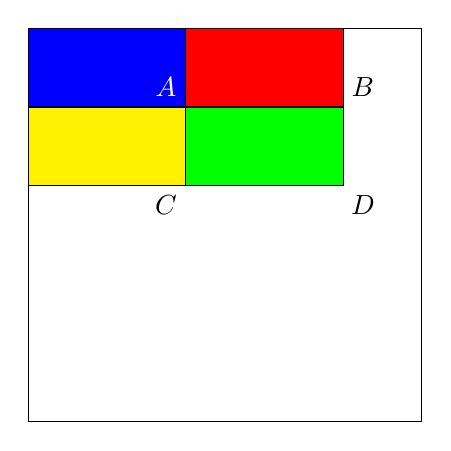
\begin{tikzpicture}
\draw (0,0) rectangle (5,5);
\draw[fill=blue] (0,5) rectangle (2,4);
\draw (1.75, 4.25)  node[white] {$A$};
\draw[fill=red] (2,5) rectangle (4,4);
\draw (4.25, 4.25)  node{$B$};
\draw[fill=yellow] (0,4) rectangle (2,3);
\draw (1.75, 2.75)  node{$C$};
\draw[fill=green] (2,4) rectangle (4,3);
\draw (4.25, 2.75)  node{$D$};
\end{tikzpicture}
\caption[Sum of area in integral image]{The sum of all values in the green area could be computed by $A+D-(C+B)$. $A$ is the sum of all pixels in the blue area, $B$ the sum of the pixels in the blue and the red areas, $C$ the sum of all pixels in the blue and yellow areas, $D$ of the green, red, blue and yellow respectively}
\label{fig:integral_image}
\end{figure}

The difference to \cite{viola2001rapid} is that one pixel at a time is represented by a complete codebook, therefore an integral image per codebook dimension has to be computed. The source image is created by adding the inverse distance of each feature patch center to its nearest cluster centroid to the corresponding codebook dimension. Afterwards, a cumulative sum over the two image axes is computed. The benefit of using integral images is that at runtime, every possible window could be computed by four reads (the corners), one sum and two subtractions between the codebooks. This reduced the computational time at the query stage to 1-2 seconds with a $500\times375$ image, 1000 codebook dimensions and 5000 windows with a 2-by-2 grid.

The downside is the memory usage, which increased dramatically. For example, a $500 \times 375 \times 1000$ integral image requires with the double datatype at least 1.4 gigabytes of data (without any meta information stored aside by matlab). The 50 images test database required therefore at least 70 gigabytes of RAM storage during the query. This also led to the problem of the time required to load the whole database. By storing it in the \MATLAB 7.3 file format, which effectively is a slightly modified HDF5 \cite{hdf5}, the program requires in average 900 seconds to load the whole database from a network shared filesystem.

This method also enabled the extraction of the query codebook from an image contained in the database without any feature or codebook computations. The reduced computational effort during the query phase consist therefore in extracting the query codebook from the database, training of the \ac{SVM}, calculating the sliding windows, extracting the codebook for each window in each image and scoring the codebooks by the trained \ac{SVM}.
% no libsvm classify

\section{Optimizing the score output}

%TODO non max suppression

The experiments showed that the \ac{SVM} output does not provide a clear separation threshold to identify positive candidates over all images in the database. The scores varied between -2 and 1 for the best matching candidates. As the candidates were most of the time correctly ordered by their visual similarity to the query image, this would not be a problem under the assumption that every image contain at least one area which is similar to the query image part. In this case, the scores could be normalized at an image level, which means that significant higher scores compared to the arithmetic mean. %TODO bild von score histogram
% gaussian fit + rho adjust

\section{Reducing the memory usage}

% kd - tree
% sparse matrix
% overwrite
% sum

\section{The framwork}
